% Appendix X

\chapter{Systematic studies}\label{app:Sys}

%----------------------------------------------------------------------------------------

\section{Systematic uncertainty associated to the stability of data over time}

The data samples used in the analysis were recorded over a period of $5$ weeks. As a quality check, the raw charged hadron multiplicities from period P$07$ and from all periods (averaged using the flux as weight) were compared. The results of this study are presented in Figs.~\ref{pic:piMultTime} to \ref{pic:pMultTime} for identified hadrons.

\newpage

\begin{sidewaysfigure}[p]
  \centering
	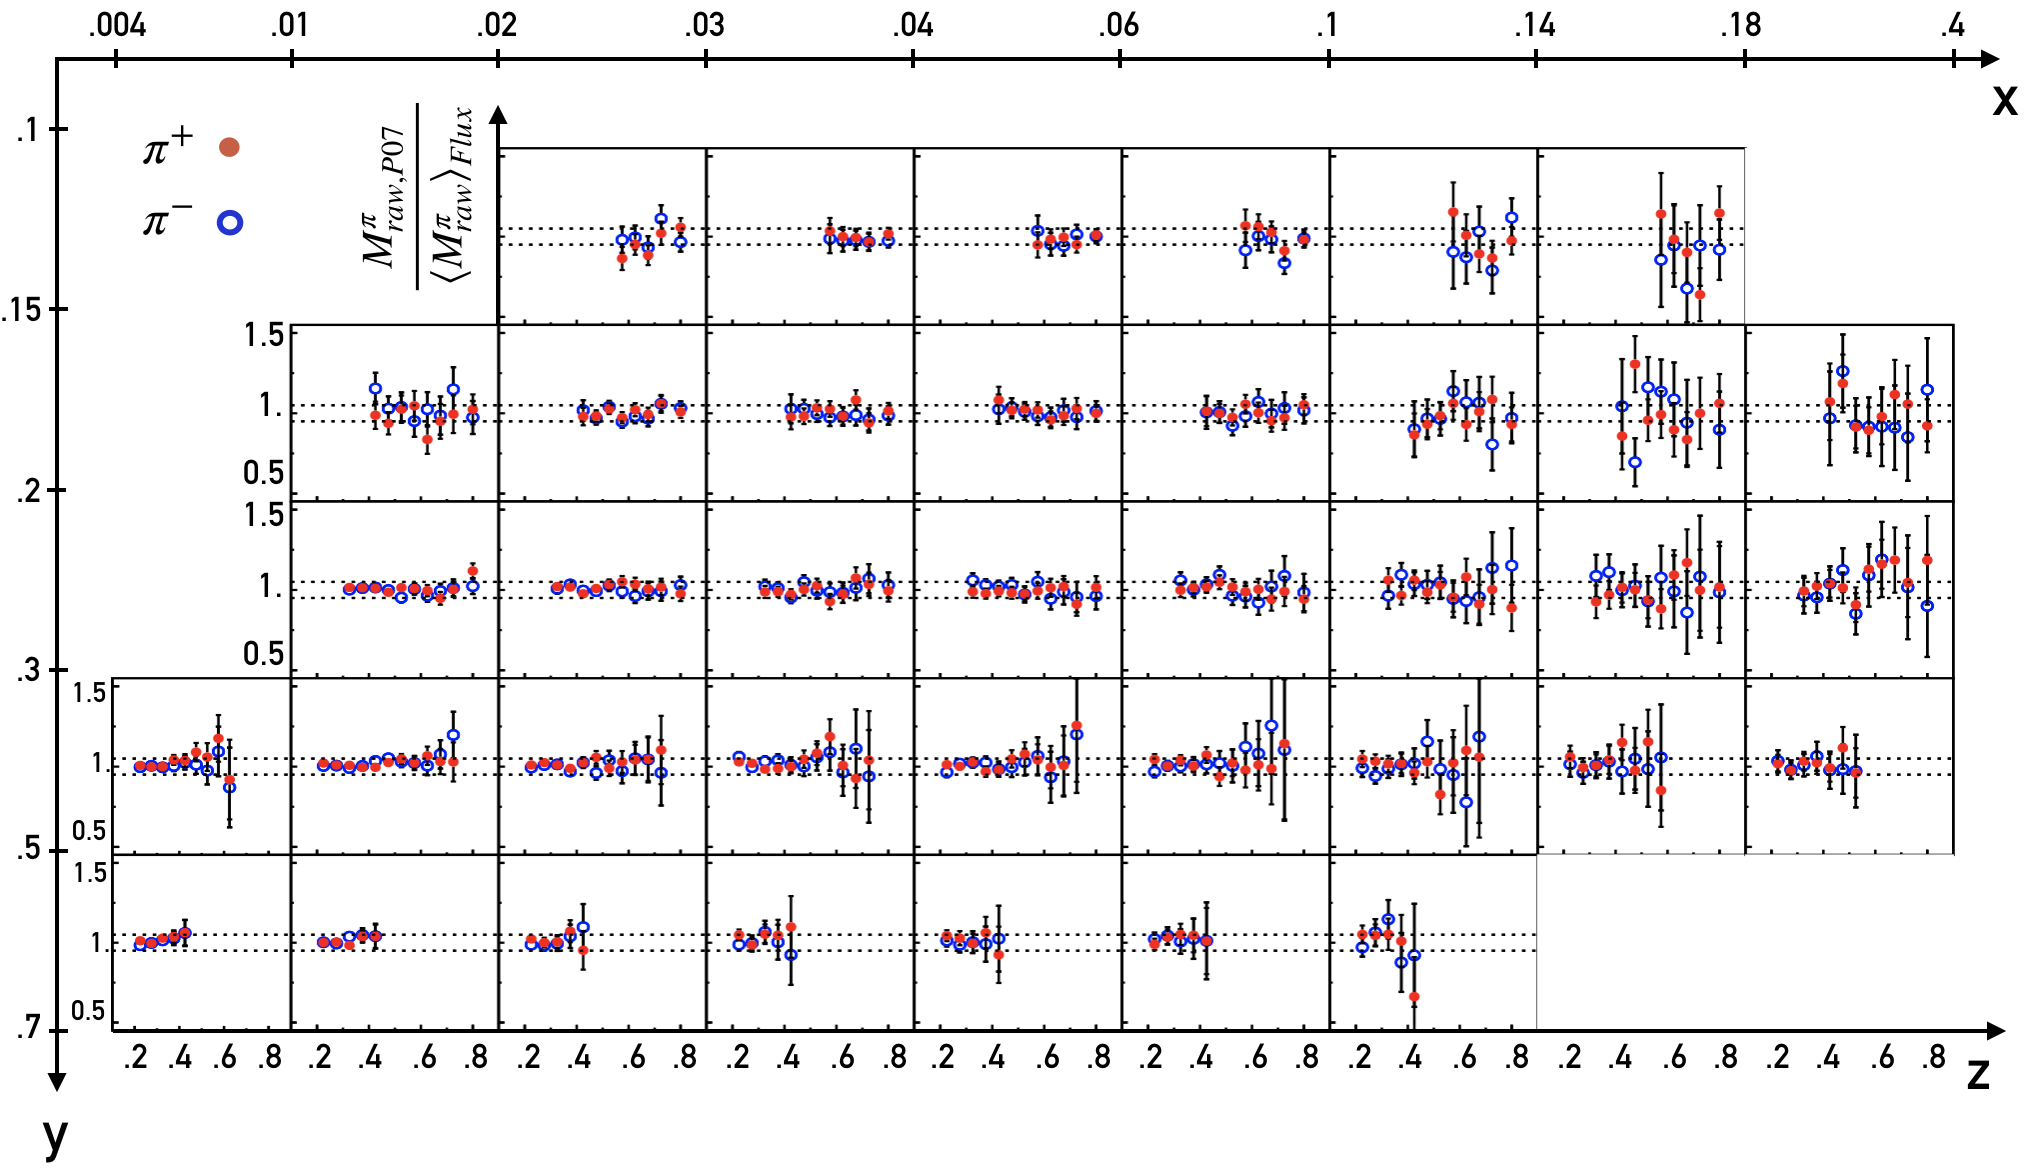
\includegraphics[scale=0.7]{./gfx/SysTimeMultpi.png}
	\caption{Same as Fig. \ref{pic:hMultTime} but for pion multiplicities.}
	\label{pic:piMultTime}
\end{sidewaysfigure}

\begin{sidewaysfigure}[p]
  \centering
	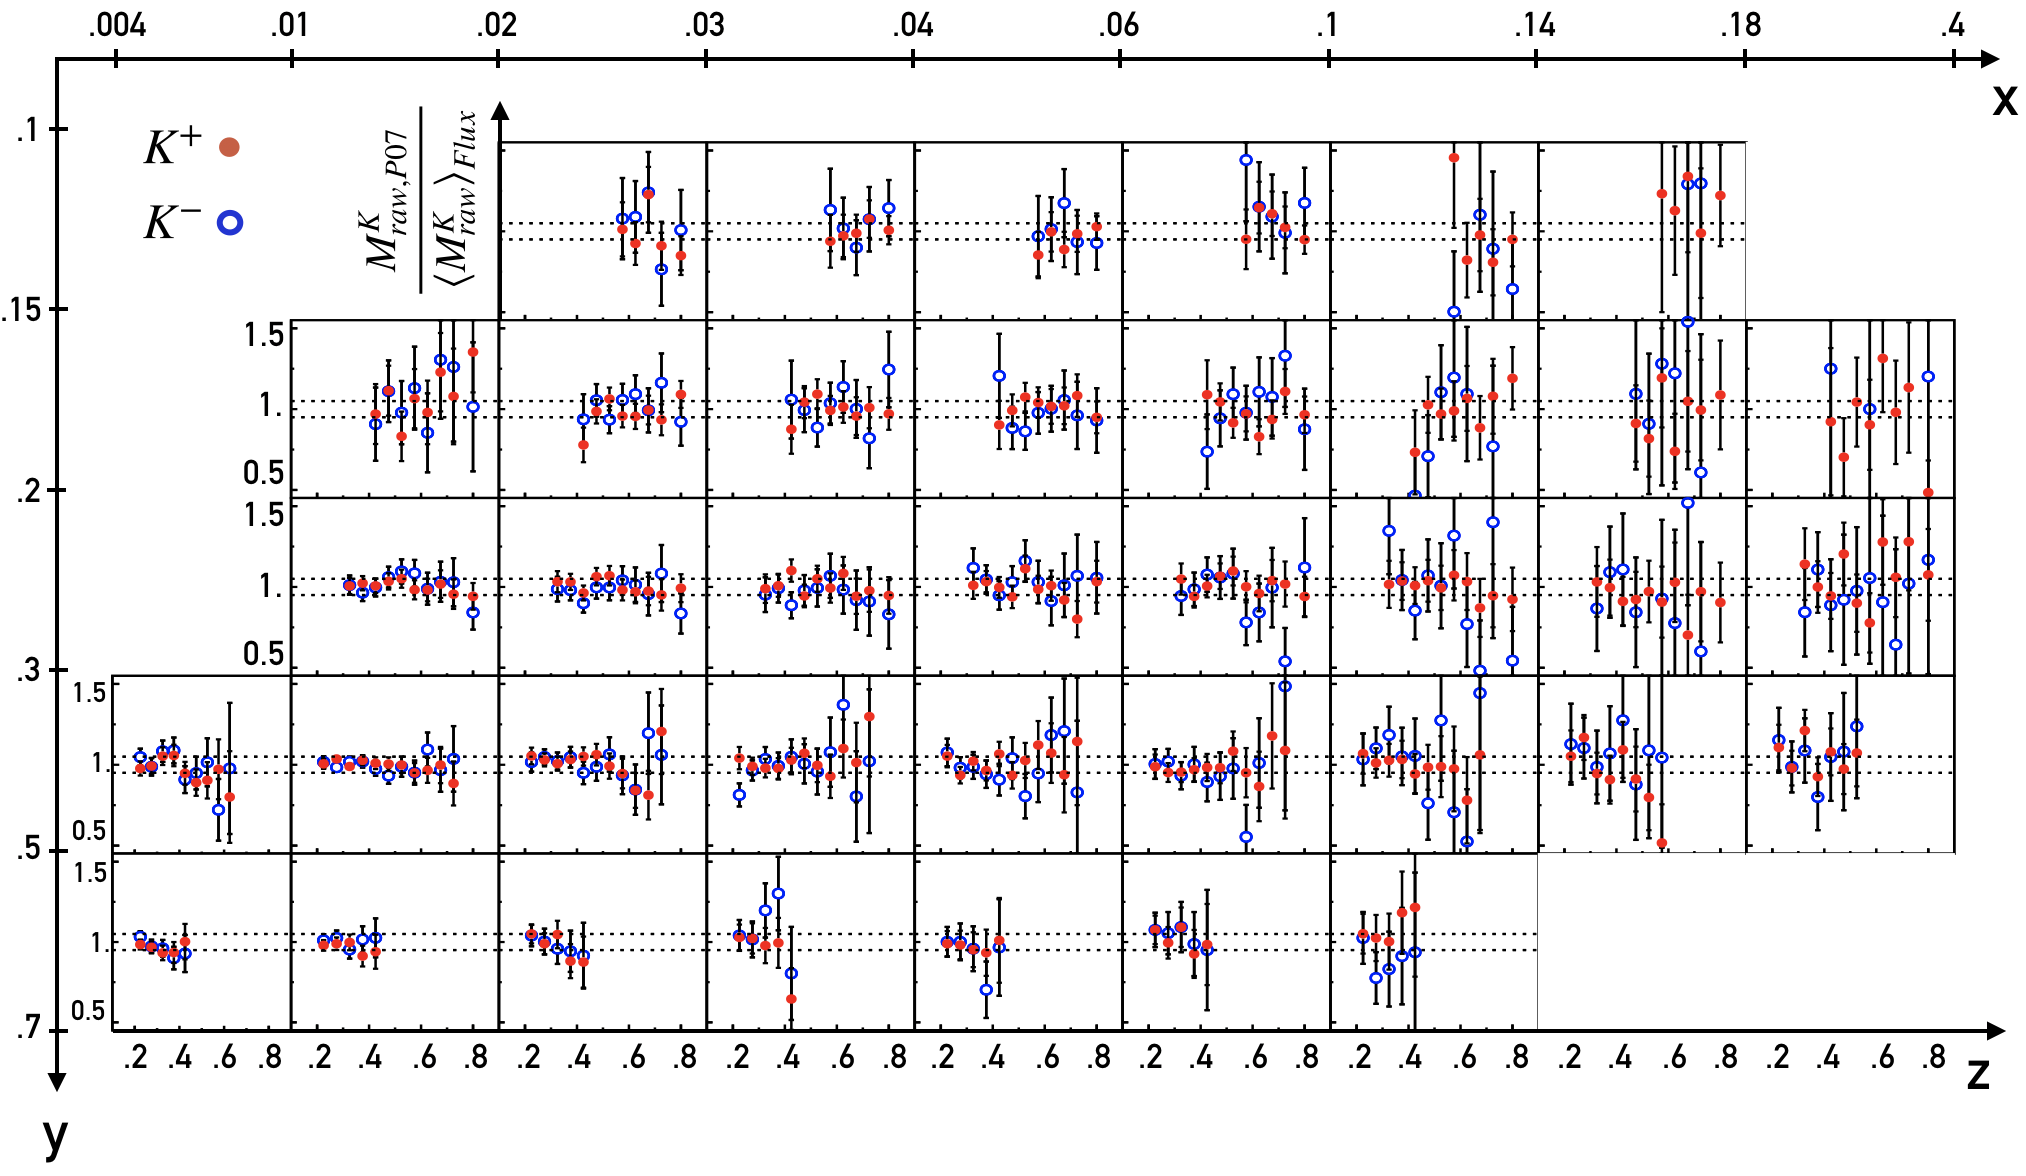
\includegraphics[scale=0.7]{./gfx/SysTimeMultk.png}
	\caption{Same as Fig. \ref{pic:hMultTime} but for kaon multiplicities.}
	\label{pic:kMultTime}
\end{sidewaysfigure}

\begin{sidewaysfigure}[p]
  \centering
	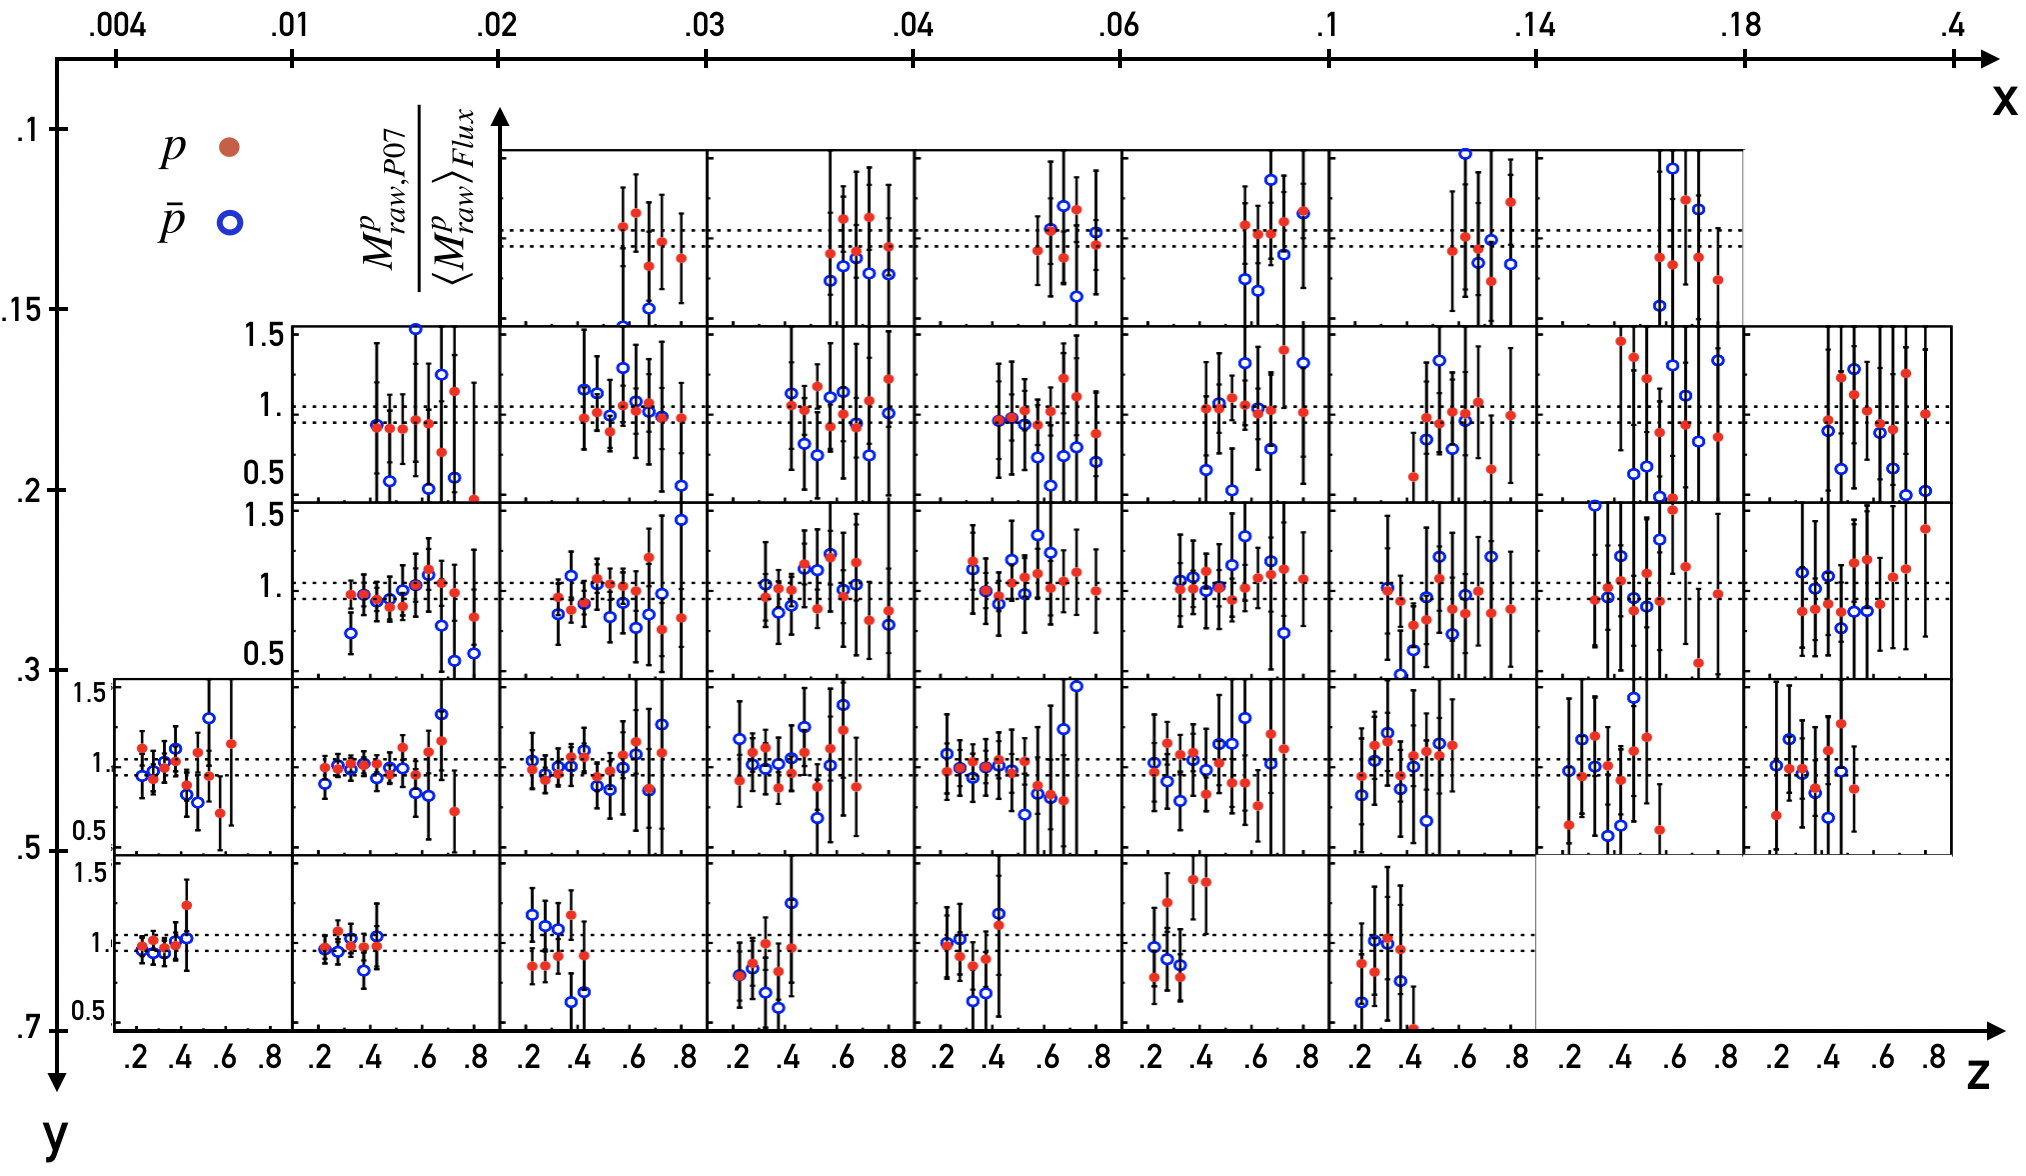
\includegraphics[scale=0.7]{./gfx/SysTimeMultp.png}
	\caption{Same as Fig. \ref{pic:hMultTime} but for proton multiplicities.}
	\label{pic:pMultTime}
\end{sidewaysfigure}
